\chapter{Aplicação de Monitoramento}
\label{chap4}

Após o detalhamento da arquitetura e dos componentes do sistema de monitoramento, este capítulo apresenta a aplicação prática da solução desenvolvida. São abordados os dois mecanismos principais responsáveis pela visualização e notificação das métricas coletadas: o dashboard e o sistema de alertas.

Na primeira seção, é detalhado o dashboard implementado, incluindo os gráficos e visualizações criados, os códigos PromQL utilizados nas consultas correspondentes e os procedimentos de processamento dos dados. A segunda seção descreve o sistema de alertas, abrangendo as regras de disparo de notificações, a configuração dos pontos e canais de contato, bem como a experiência prática obtida com os diferentes sistemas de alertas disponíveis no ecossistema adotado. A terceira seção apresenta um caso de uso prático, ilustrando a aplicação do sistema de monitoramento em um cenário real.

\section{Dashboard}
\label{section:Dashboard}

Conforme mencionado ao longo deste trabalho, os princípios de IaC são fundamentais para assegurar a reprodutibilidade e o versionamento de toda a infraestrutura desenvolvida. Essa abordagem abrange não apenas os componentes centrais do projeto, mas também os dashboards e sistemas de alertas configurados. Por meio de arquivos declarativos YAML, são definidas e versionadas as configurações internas, o processamento de dados, as consultas PromQL e as regras de alertas (conforme será detalhado na Seção \ref{section:Alertas}), automatizando integralmente o fluxo de trabalho.

A configuração do Prometheus como fonte de dados padrão do Grafana foi realizada através do arquivo \verb|datasource.yaml|, enquanto as configurações internas específicas do dashboard foram estabelecidas no arquivo \verb|dashboards.yml|, conforme apresentado nos Códigos Fonte \ref{lst:default-datasource} e \ref{lst:dashboards-yml}, respectivamente.

\begin{lstlisting}[caption={Arquivo datasource.yml}, label={lst:default-datasource}]
apiVersion: 1
datasources:
- name: Prometheus
  type: prometheus
  access: proxy
  url: http://prometheus:9090
  isDefault: true
\end{lstlisting}

\begin{lstlisting}[caption={Arquivo dashboards.yml}, label={lst:dashboards-yml}]
apiVersion: 1
providers:
  - name: 'monitoring'
    orgId: 1
    folder: 'Monitoring'
    type: file
    disableDeletion: false
    updateIntervalSeconds: 5
    options:
      path: /etc/grafana/dashboards
      foldersFromFilesStructure: false
\end{lstlisting}

Para o processamento dos dados, adotou-se uma abordagem híbrida: a normalização dos dados foi implementada por meio de consultas PromQL estruturadas em arquivos YAML e executadas como \verb|Recording Rules| diretamente no Prometheus, enquanto as consultas específicas de cada gráfico foram definidas na interface web do Grafana.

O cenário ótimo consistiria na utilização exclusiva de \texttt{Recording Rules} para todo o processamento de dados, uma vez que as consultas PromQL executadas pelo Grafana seguem o fluxo: Grafana \foreign{frontend} $\rightarrow$ Grafana \foreign{backend} $\rightarrow$ Prometheus, retornando subsequentemente pelos mesmos componentes em ordem inversa para entregar os resultados de cada consulta. Em contrapartida, as \verb|Recording Rules| realizam o processamento internamente no Prometheus (exemplo de benefício do TSDB), otimizando o desempenho.

Embora computacionalmente mais eficientes, as \texttt{Recording Rules} apresentam limitações operacionais como a incompatibilidade com as variáveis dinâmicas do Grafana (\verb|Grafana Variables|) e a necessidade de reinicialização do Prometheus para aplicar modificações nas regras. Diante destas restrições, a abordagem híbrida oferece maior praticidade e conveniência para o desenvolvimento de dashboards, ainda que implique em um custo computacional superior.

Na normalização dos dados no Prometheus, são realizadas duas operações principais, quando aplicáveis: a conversão de métricas com diferentes unidades (como microssegundos, bytes, contagens) para formatos padronizados, como percentuais; e a transformação de métricas provenientes de diferentes hosts para um formato consistente, possibilitando comparações e visualizações agregadas.

Um exemplo prático dessa normalização é a métrica de uso de CPU "Carga de usuário" no host físico, ela representa uma porcentagem de utilização por tempo total, enquanto nos dispositivos virtuais é expressa como um valor acumulado em microssegundos desde a inicialização do contêiner correspondente. Para unificar essas métricas, utiliza-se a consulta PromQL apresentada no Código Fonte \ref{lst:cpu_user_load}. Além disso, esta normalização incluiu a padronização e otimização de labels, e a unificação das métricas numa única métrica consolidada: \verb|cpu_user_load|.

As funções \verb|label_replace| são empregadas para manipular as labels, enquanto a função \verb|irate| calcula a taxa de variação das duas amostras mais recentes da janela de tempo definida --- neste caso, 30 segundos, conforme a frequência de Nyquist. Essa taxa é convertida de microssegundos para segundos por meio da divisão por $10^{6}$ e, em seguida, multiplicada por 100 para obter o valor em percentual.

A métrica final \verb|cpu_user_load| é, então, utilizada nos gráficos do Grafana, oferecendo uma visão integrada do uso de CPU tanto para hosts físicos quanto para contêineres.

A escolha da função \verb|irate|, que calcula a taxa instantânea de variação, em detrimento da função \verb|rate|, que calcula a taxa média ao longo do intervalo, deve-se à necessidade de detectar variações rápidas, como picos de uso de CPU, que poderiam ser suavizados pela média.

\begin{lstlisting}[caption={Arquivo cpu.yml}, label={lst:cpu_user_load}]
groups:
  - name: cpu_normalization
    rules:
      - record: cpu_user_load
        expr: >
          label_replace(
            label_replace(
              irate(container_cgroup_cpu_stat_user_usec
              {job="virtual_hosts"}[30s]) 
              / 1e6 * 100,
              "instance", "", "", ""
            ),
            "path", "", "", ""
          )
        labels:
          unit: percent
      [...]
      - record: cpu_user_load
        expr: >
          label_replace(
            label_replace(
              physical_cpu_usage_user{job="physical_host"},
              "instance", "", "", ""
            ),
            "cpu", "", "", ""
          )
        labels:
          unit: percent
\end{lstlisting}

\newpage

\begin{lstlisting}[caption={Métricas de CPU \myenquote{Carga de usuário} pré-normalização}, label={lst:telegraf-cpu-user-load}]
  physical_cpu_usage_user{alias="Host Machine", cpu="cpu-total", host="6RW9K03", instance="172.17.0.1:9273", job="physical_host"}	16.283422459908643

  container_cgroup_cpu_stat_user_usec{alias="Ubuntu 1", host="device1", instance="device_1:9273", job="virtual_hosts", path="/sys/fs/cgroup/"}
     32102389
\end{lstlisting}

\begin{lstlisting}[caption={Métricas de CPU \myenquote{Carga de usuário} normalizadas}, label={lst:normalized-cpu-user-load}]
  cpu_user_load{alias="Host Machine", host="6RW9K03", job="physical_host", unit="percent"}	5.620946432860638 
  cpu_user_load{alias="Ubuntu 1", host="device1", job="virtual_hosts", unit="percent"}	
     0.59546
\end{lstlisting}

O restante dos arquivos de \verb|Recording Rules| do Prometheus podem ser encontrados no repositório do projeto \citep{vitorcossetti2025}, na pasta \verb|configs/prometheus/rules|.

Seguindo a abordagem híbrida e após o processamento dos dados no Prometheus, inicia-se a construção dos dashboards por meio da interface web do Grafana. Inicialmente, são criadas as \verb|Grafana Variables|, que atuam como filtros globais para todos os gráficos, permitindo a seleção dinâmica de parâmetros para uma visualização e interpretação mais eficientes dos dados. As variáveis configuradas estão listadas na Tabela \ref{tab:grafana-variables}:

\begin{table}[H]
\centering
\caption{Grafana Variables.}
\label{tab:grafana-variables}
\begin{tabular}{cl}
\toprule
\textbf{Variável} & \textbf{Filtro aplicado} \\
\midrule
\verb|Job| & Categoria do dispositivo (físico ou virtual) \\
\verb|Device| & Dispositivo (nome do host físico ou virtual) \\
\verb|Disk Partition| & Partição de disco (exemplo: \verb|/dev/sda1|) \\
\verb|Network Interface| & Interface de rede (exemplo: \verb|eth0|, \verb|wlan0|) \\
\bottomrule
\end{tabular}
\end{table}

Outra configuração global relevante refere-se aos intervalos de atualização e tempo aplicados a todos os gráficos. O intervalo de atualização define a frequência com que os dados são atualizados, enquanto o período temporal especifica o intervalo de tempo exibido nos gráficos. Embora esses parâmetros possam ser ajustados conforme a necessidade do usuário, para garantir um monitoramento próximo ao tempo real e sincronizado com as configurações de scraping do Telegraf e do Prometheus, o intervalo de atualização foi definido para 5 segundos e o período temporal para 5 minutos. Adicionalmente, tais valores podem ser modificados individualmente para cada gráfico, sendo que as configurações específicas prevalecem sobre as globais.


\begin{figure}[ht]
\centering
\setlength{\abovecaptionskip}{-20pt}
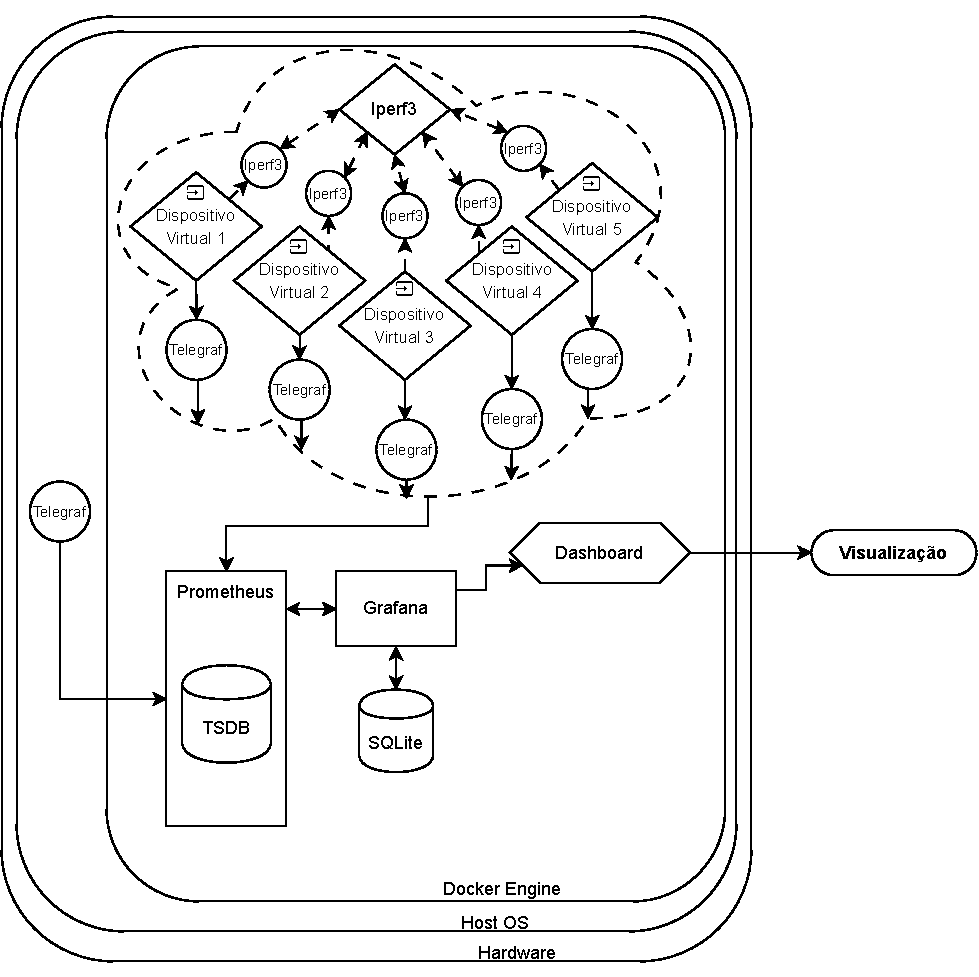
\includegraphics[width=\textwidth]{Imagens/chap04/by-blocks/dashboard_diagram.pdf}
\caption{Visualização.}
\label{fig:DiagramaVisualizacao}
\end{figure}



\section{Alertas e Notificações}
\label{section:Alertas}


\section{Caso de Uso}
\label{section:CasosDeUso}

Um caso de uso para este projeto é o monitoramento da saturação dos equipamentos do próprio autor. Com o dashboard e notificações de alertas desenvolvidos nestre trabalho, foi possível identificar causadores de travamentos, como picos de \myenquote{Aguardo de I/O} da CPU e \myenquote{Utilização I/O} de disco quando executando os testes de saturação dos contêineres de forma assíncrona, o que motivou para a mudança para a execução síncrona dos testes, conforme detalhado em \ref{subsection:TestesSaturacao}.

% foram feitas tentativas de utilização de ferramentas de \foreign{chaos-engineering} como Pumba e ChaosBlade e até mesmo tentativas de manipulação direta de iptables para gerar tráfego de rede, mas essas ferramentas não se mostraram adequadas para este trabalho.

% Por debaixo dos panos, ferramentas de \foreign{chaos testing} utilizam para testes de rede o módulo \verb|netem| do sistema de controle de tráfego \verb|tc| do Linux. Esse sistema opera na camada de controle de tráfego (\verb|qdisc|). Enquanto isso, o \foreign{plugin} \verb|inputs.net| do Telegraf a partir da leitura do \verb|procfs/net/dev|, que se encontra na camada de interface de rede. Ou seja, 

{\color{blue}
\section{Dashboard}

\begin{enumerate}  
  \item OK $\rightarrow$ comentar sobre sobre as coisas que o provisioning já adiantou (datasource padrão, por exemplo);
  \item OK $\rightarrow$ a normalização dos dados usando o Pormetheus Recording Rules
  \item OK $\rightarrow$ Criação dos filtros globais (Grafana Variables);
  \item OK $\rightarrow$ Regras globais (span e refresh rate);
  \item Falar de cada gráfico, justificando visualizações, comentando sobre as queries/cálculos e colocar imagens;
  \item Quando chegar em CPU, explicar o porquê de haver picos acima de 100\% mesmo com a limitação de cpu (olhar pasta docs/cpu\_shares)
  \item Quando chegar na seção de disco, apresentar o estudo de caĺculo do df (motivação e resultados);
  \item Chegando na parte de redes, justificar o porquê de nao termos dados de drop e erro de pacotes (apresentar o estudo de caso de camadas de rede e aplicação);
  \item Fechamento explicando a exportação do JSON e seu versionamento e carregamento automatico via docker volume;
\end{enumerate}


\section{draft-Alertas e Notificações}
\label{section:draft-Alertas}
\begin{enumerate}
  \item Comentar sobre o Alertmanager e a sua configuração;
  \item Explicar como adicionei o servidor smtp do gmail e as tentativas falhas com o Telegram;
  \item Configuração das regras de notificação e os pontos de contato;
  \item Como utilizei, a primeiro momenot, a UI do Grafana para criar os alertas (isso era interessante pq vinculava automaticamente o alerta ao respectivo gráfico);
  \item Como, assim como no dashboard, eu exportava e versionava tudo via JSON;
  \item Problemas do SQLite e a migração para o Postgres e dps para MYSQL (explicitar como a migração foi fácil graças ao provisionamento, versionamento, uso do Docker e TSDB fazendo o trabalho de persistência);
  \item Migração para o Alertmanager+TSDB (enfatizar como tudo fica embutido no Prometheus e como isso simplifica a arquitetura);
  \item Em algum lugar mencionar o Granafa Unified Alerting ser capaz de interpretar o alerts.yml do prometheus e automaticamente criar os alertas Grafana-Managed
  \item Mencionar em algum lugar que a primeira configuração do mysql demorou mto (188s)
\end{enumerate}


}



\begin{figure}[H]
\centering
\setlength{\abovecaptionskip}{-20pt}
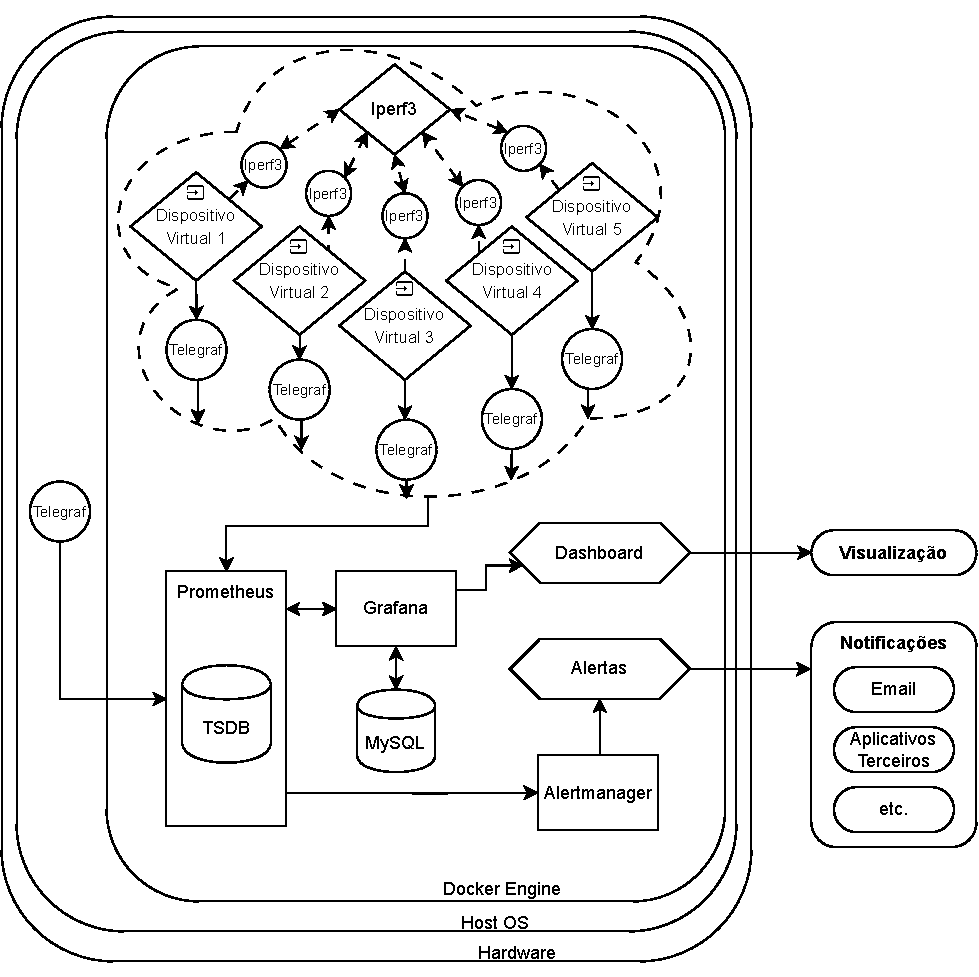
\includegraphics[width=\textwidth]{Imagens/chap04/by-blocks/alerts_diagram.pdf}
\caption{Notificações e Arquitetura Final.}
\label{fig:DiagramaAlertas}
\end{figure}


\begin{figure}[H]
\centering
\setlength{\abovecaptionskip}{-20pt}
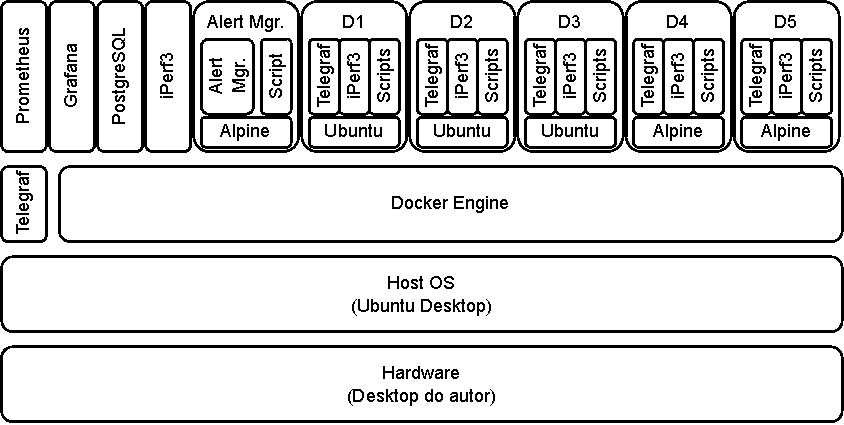
\includegraphics[width=\textwidth]{Imagens/chap04/final_stack.pdf}
\caption{\foreign{Stack} final.}
\label{fig:StackFinal}
\end{figure}

